%!TEX root = ../main.tex
%%

\chapter{Testing}
The project's terminal goal of reliable cell counting can be evaluated by the artefact's numerical and percentage count error. Since a detection and localisation network was used, the instrumental goal of the project is to accurately detect and localise cells (in order that they can be counted), and the detection and localisation performance of the underlying model can provide insights into whether the artefact's counts are reached empirically or merely accidentally. The data captured by Weights and Biases during training of a YOLOv5 model includes many metrics for the detection and localisation performance of the model, and provides ample material for qualitative and quantitative evaluation.

\section{Summary}
\subsection{Counting}
Counting accuracy generally improved with each experiment, with the notable exception of Model 2, whose count error was significantly higher than Model 1. Eventually a mean numerical error of 15 and percentage error of around 18\% was achieved by Model 7, the best so far. The counting performance for each model can be seen in Table \ref{count_error}, and Figures \ref{num_error} and \ref{pct_error}.\\

With the exception of Model 1, all models consistently counted more than the ground truth (see Tables \ref{count_1} to \ref{count_7} in the appendix). This was in keeping with the constraint that overcounting is more desirable than undercounting in this use case.\\

\begin{table}
\centering
\begin{tabular}{ |l||l|l|  }
\hline
\multicolumn{5}{|c|}{Count Error} \\
\hline
Model & Num. Error & Pct. Error \\
\hline
1 &      74.25 &   90.767435 \\
2 &      87.00 &  103.001947 \\
3 &      83.25 &  101.850956 \\
4 &      63.00 &   75.363021 \\
5 &      62.50 &   77.071071 \\
6 &      16.00 &   20.892626 \\
\textbf{7} &      \textbf{15.00} &   \textbf{18.237132}\\
\hline
\end{tabular}
\caption{Count error for all models (numerical and percentage)}
\label{count_error}
\end{table}

\begin{figure}[h!]
	\centering
	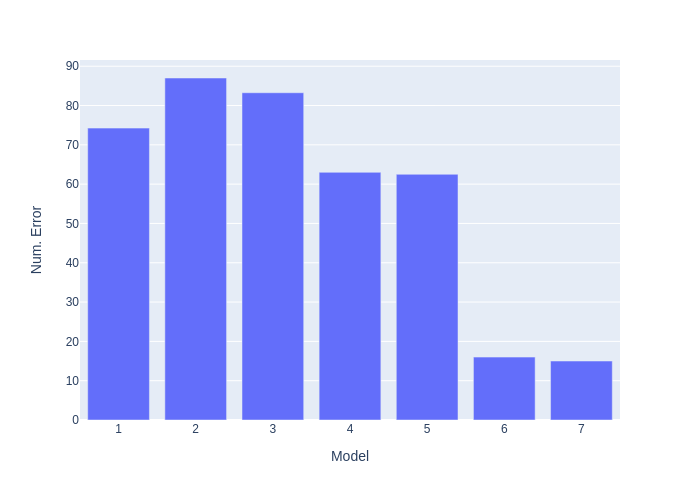
\includegraphics[width=0.8\textwidth]{images/05Testing/num_error.png}
	\caption{Numerical error by model}
	\label{num_error}
\end{figure}

\begin{figure}[h!]
	\centering
	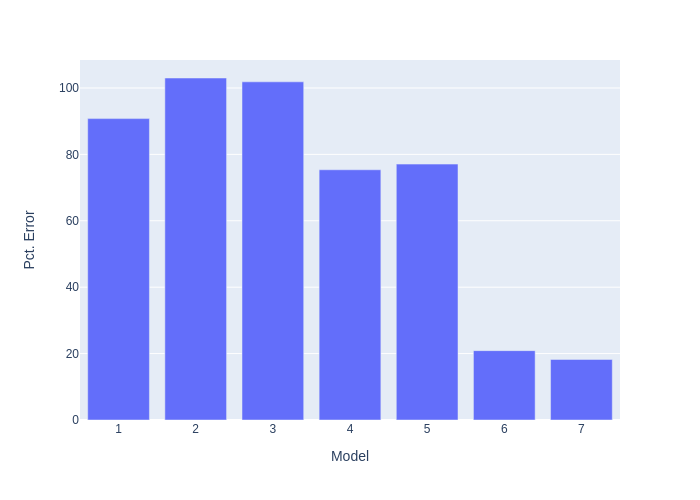
\includegraphics[width=0.8\textwidth]{images/05Testing/pct_error.png}
	\caption{Percentage error by model}
	\label{pct_error}
\end{figure}

\subsection{Metrics}
YOLOv5 produces several metrics to keep track of object detection and localisation performance\footnote{COCO - Common Objects in Context. (no date). Available at: https://cocodataset.org/#detection-eval (Accessed: 05/05/2022).}:\\

\begin{enumerate}
    \item \verb`mAP\_0.5:0.95` (mean average precision for all IoU thresholds from 0.5 to 0.95, step 0.05)
    \item \verb`mAP\_0.5` (mAP at IoU threshold 0.5)
    \item \verb`precision`
    \item \verb`recall`
\end{enumerate}

It was observed during experimentation that YOLOv5's metrics for detection and localisation were of limited relevance in the cell counting task. There was little difference in these metrics between models, despite dramatic changes in count error. In addition, these metrics did not indicate a trend of continuous improvement: some later models' metrics were inferior to those of earlier models which had higher count error. Metrics generally suggested that the models were performing better than their count error and predicted bounding boxes indicated. Notably, mAP metrics improved after Model 1, but this corresponded with a dramatic rise in false positives. It may be the case that increasing mAP simply a result of more false positives.

recall was expected to be far lower for Model 1—which produced a nearly 100\% false negative rate—and precision to be much lower for subsequent models, which produced false positive rates of over 50\%.\\

Initially, the number of epochs was kept low to avoid overfitting, but a key insight gleaned from the model metrics is that training for more epochs does not cause detection and localisation performance to degrade due to overfitting, even after 300 epochs (see Figures \ref{map_0.95}, \ref{map_0.5}, \ref{precision}, and \ref{recall}). In fact, increasing the number of training epochs resulted in dramatic improvements in counting performance.

https://github.com/ultralytics/yolov5/issues/5760

\begin{table}
\centering
\begin{tabular}{ |l||l|l|l|l|  }
\hline
\multicolumn{3}{|c|}{Performance metrics} \\
\hline
Model & mAP\_0.5:0.9 & mAP\_0.5 & precision & recall \\
\hline
1 &      0.44 &   0.77 & 0.77 & 0.68\\
2 &      0.48 &  0.85 & \textbf{0.88} & 0.74 \\
3 &      0.51 &  \textbf{0.91} & \textbf{0.88} & \textbf{0.84} \\
4 &      0.54 & 0.89 & \textbf{0.88} & 0.83 \\
5 &      0.56 & 0.88 & \textbf{0.88} & 0.83 \\
6 &      0.56 & 0.88 & 0.87 & 0.79 \\
7 &      \textbf{0.57} & 0.87 & \textbf{0.88} & 0.82\\
\hline
\end{tabular}
\caption{Performance metrics for all models}
\label{metrics}
\end{table}

\begin{figure}[h!]
	\centering
	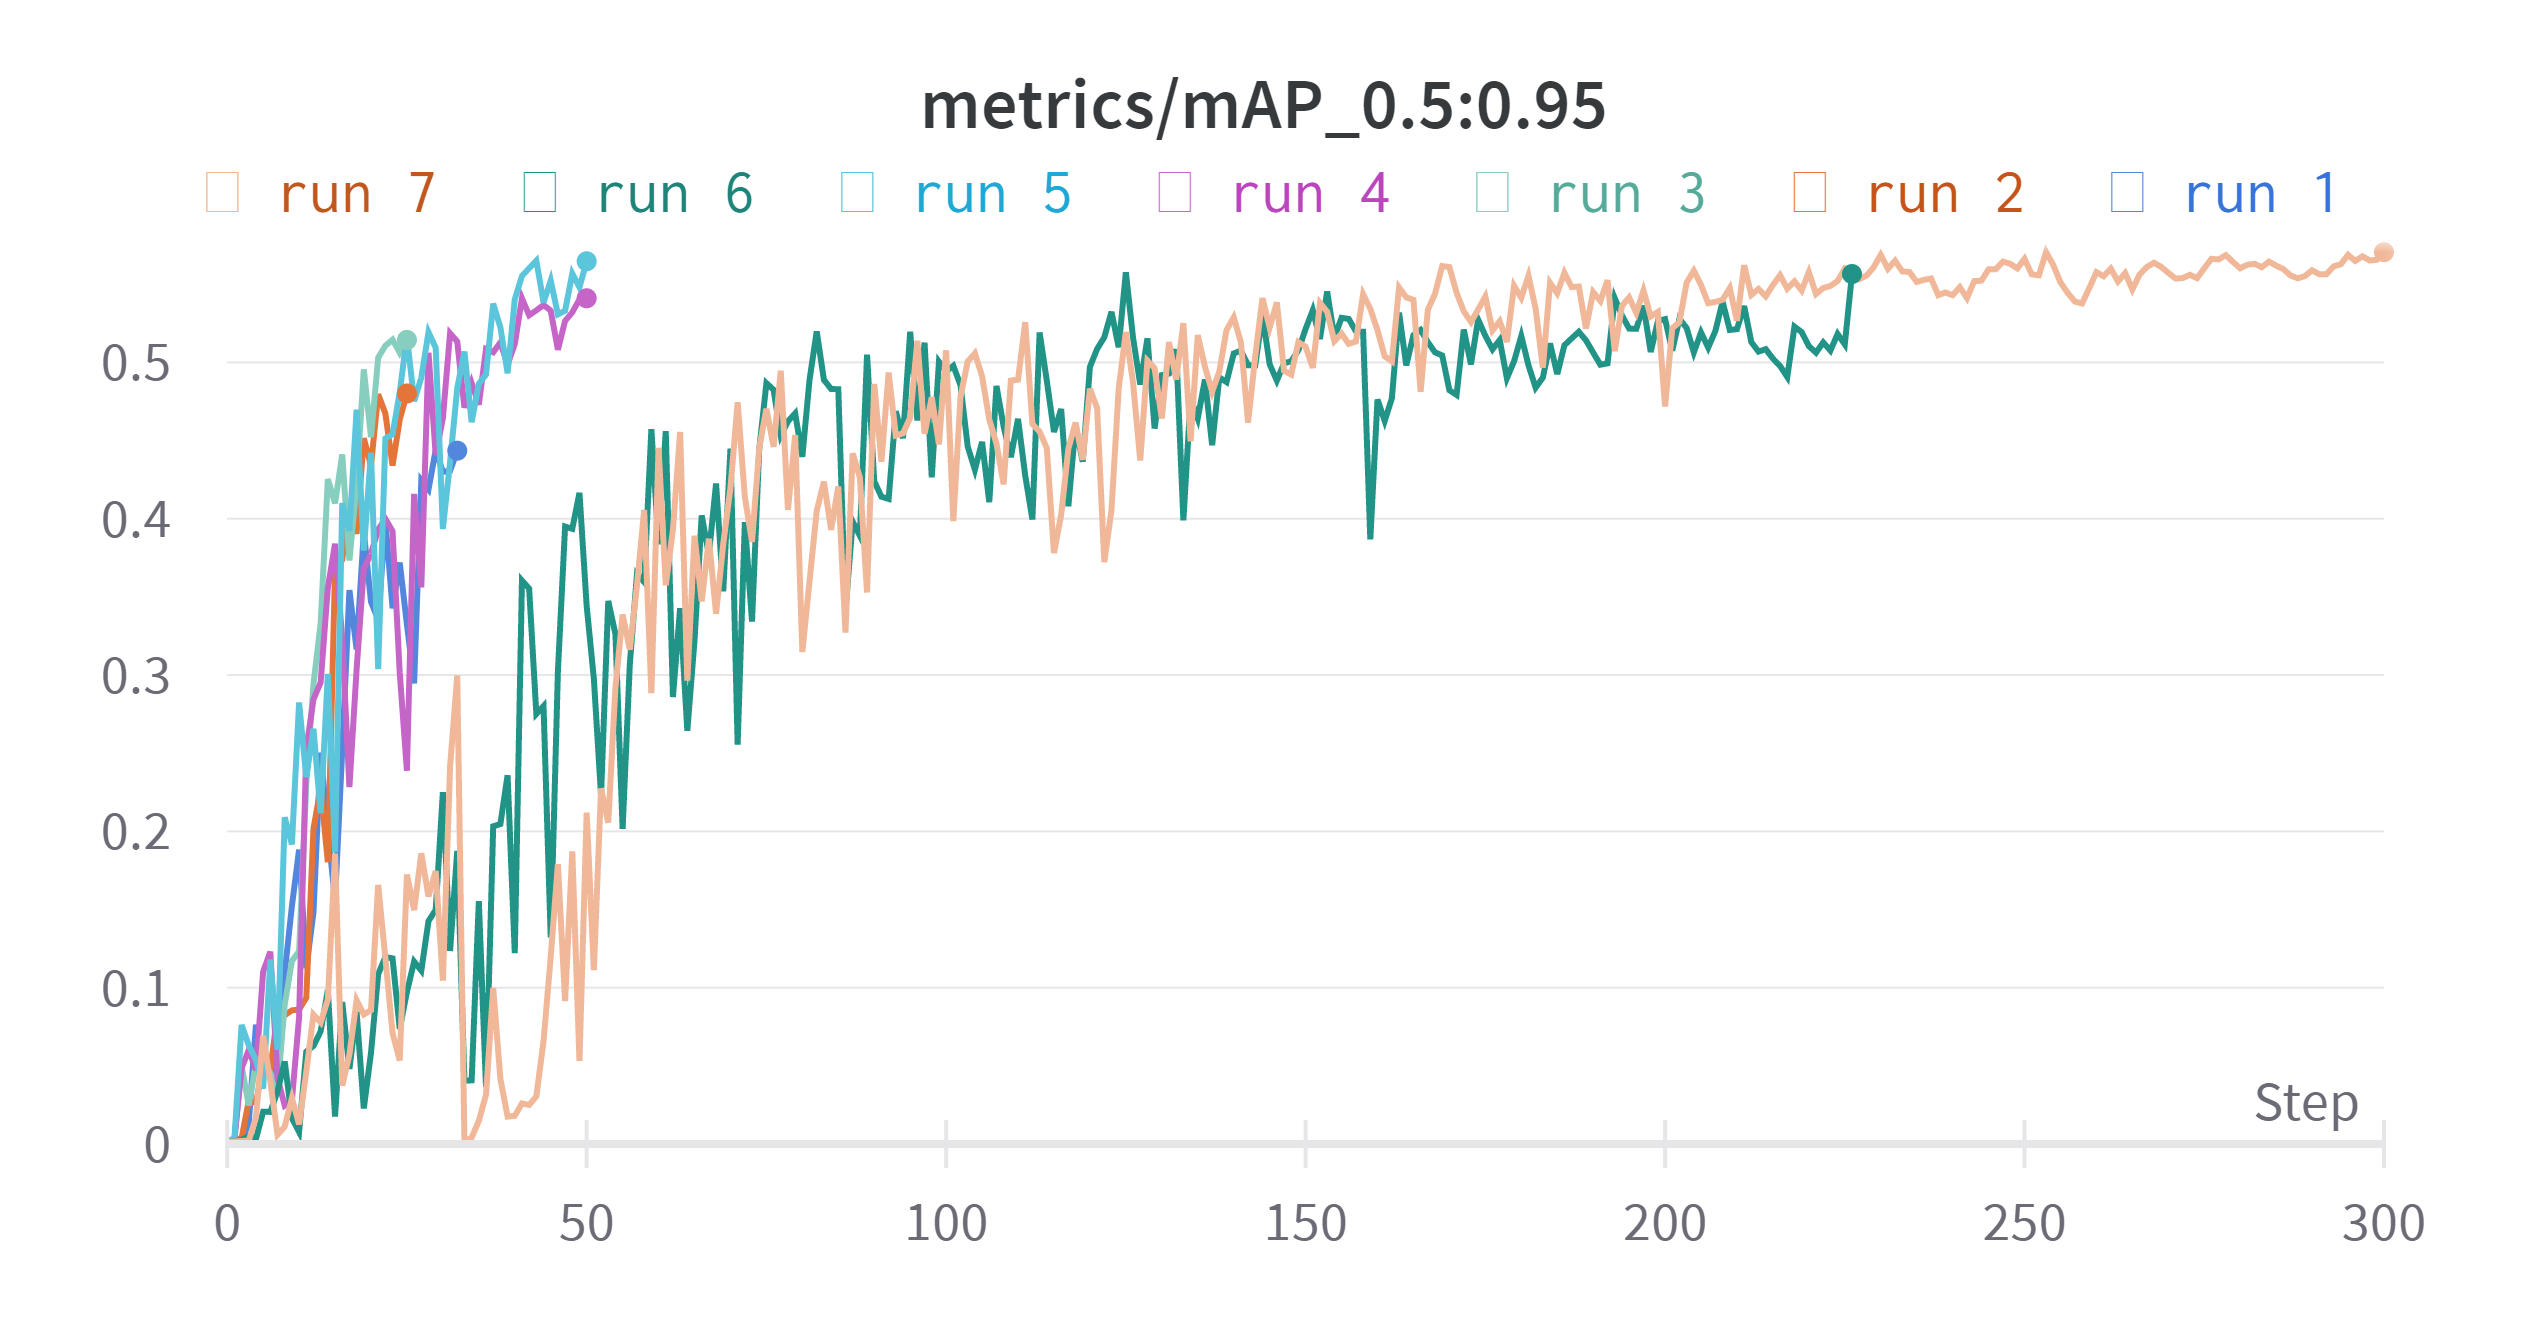
\includegraphics[width=0.8\textwidth]{images/05Testing/map_0.95.png}
	\caption{mAP\_0.5:0.95}
	\label{map_0.95}
\end{figure}

\begin{figure}[h!]
	\centering
	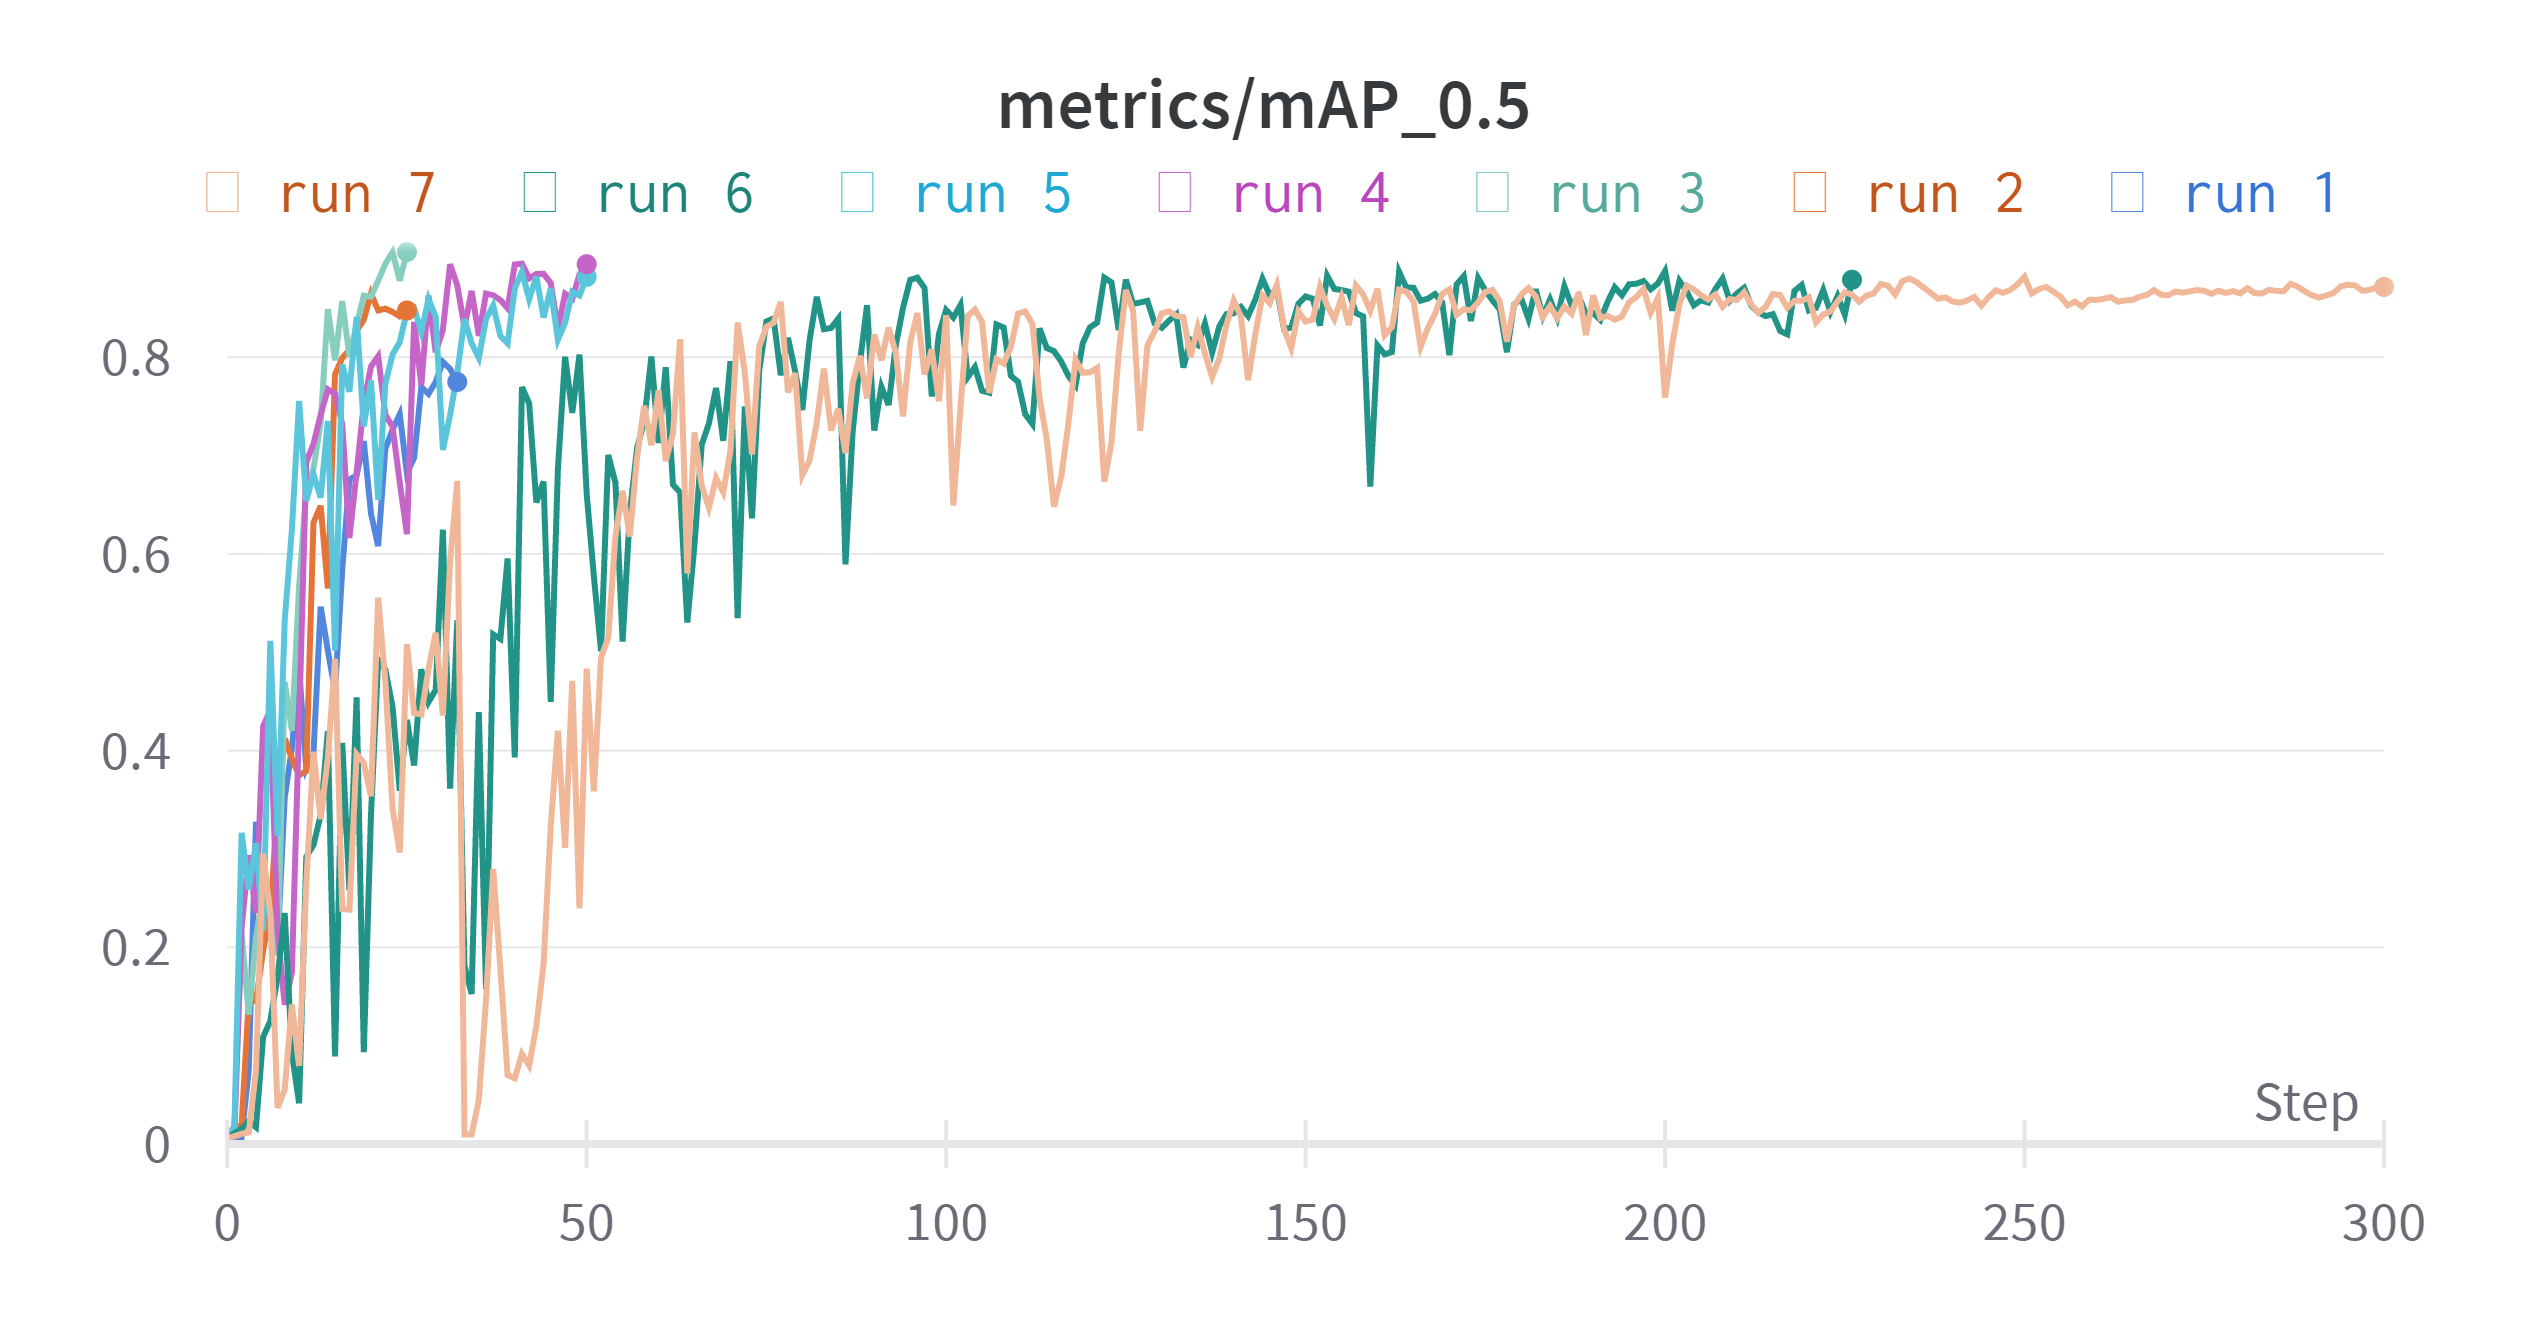
\includegraphics[width=0.8\textwidth]{images/05Testing/map_0.5.png}
	\caption{mAP\_0.5}
	\label{map_0.5}
\end{figure}

\begin{figure}[h!]
	\centering
	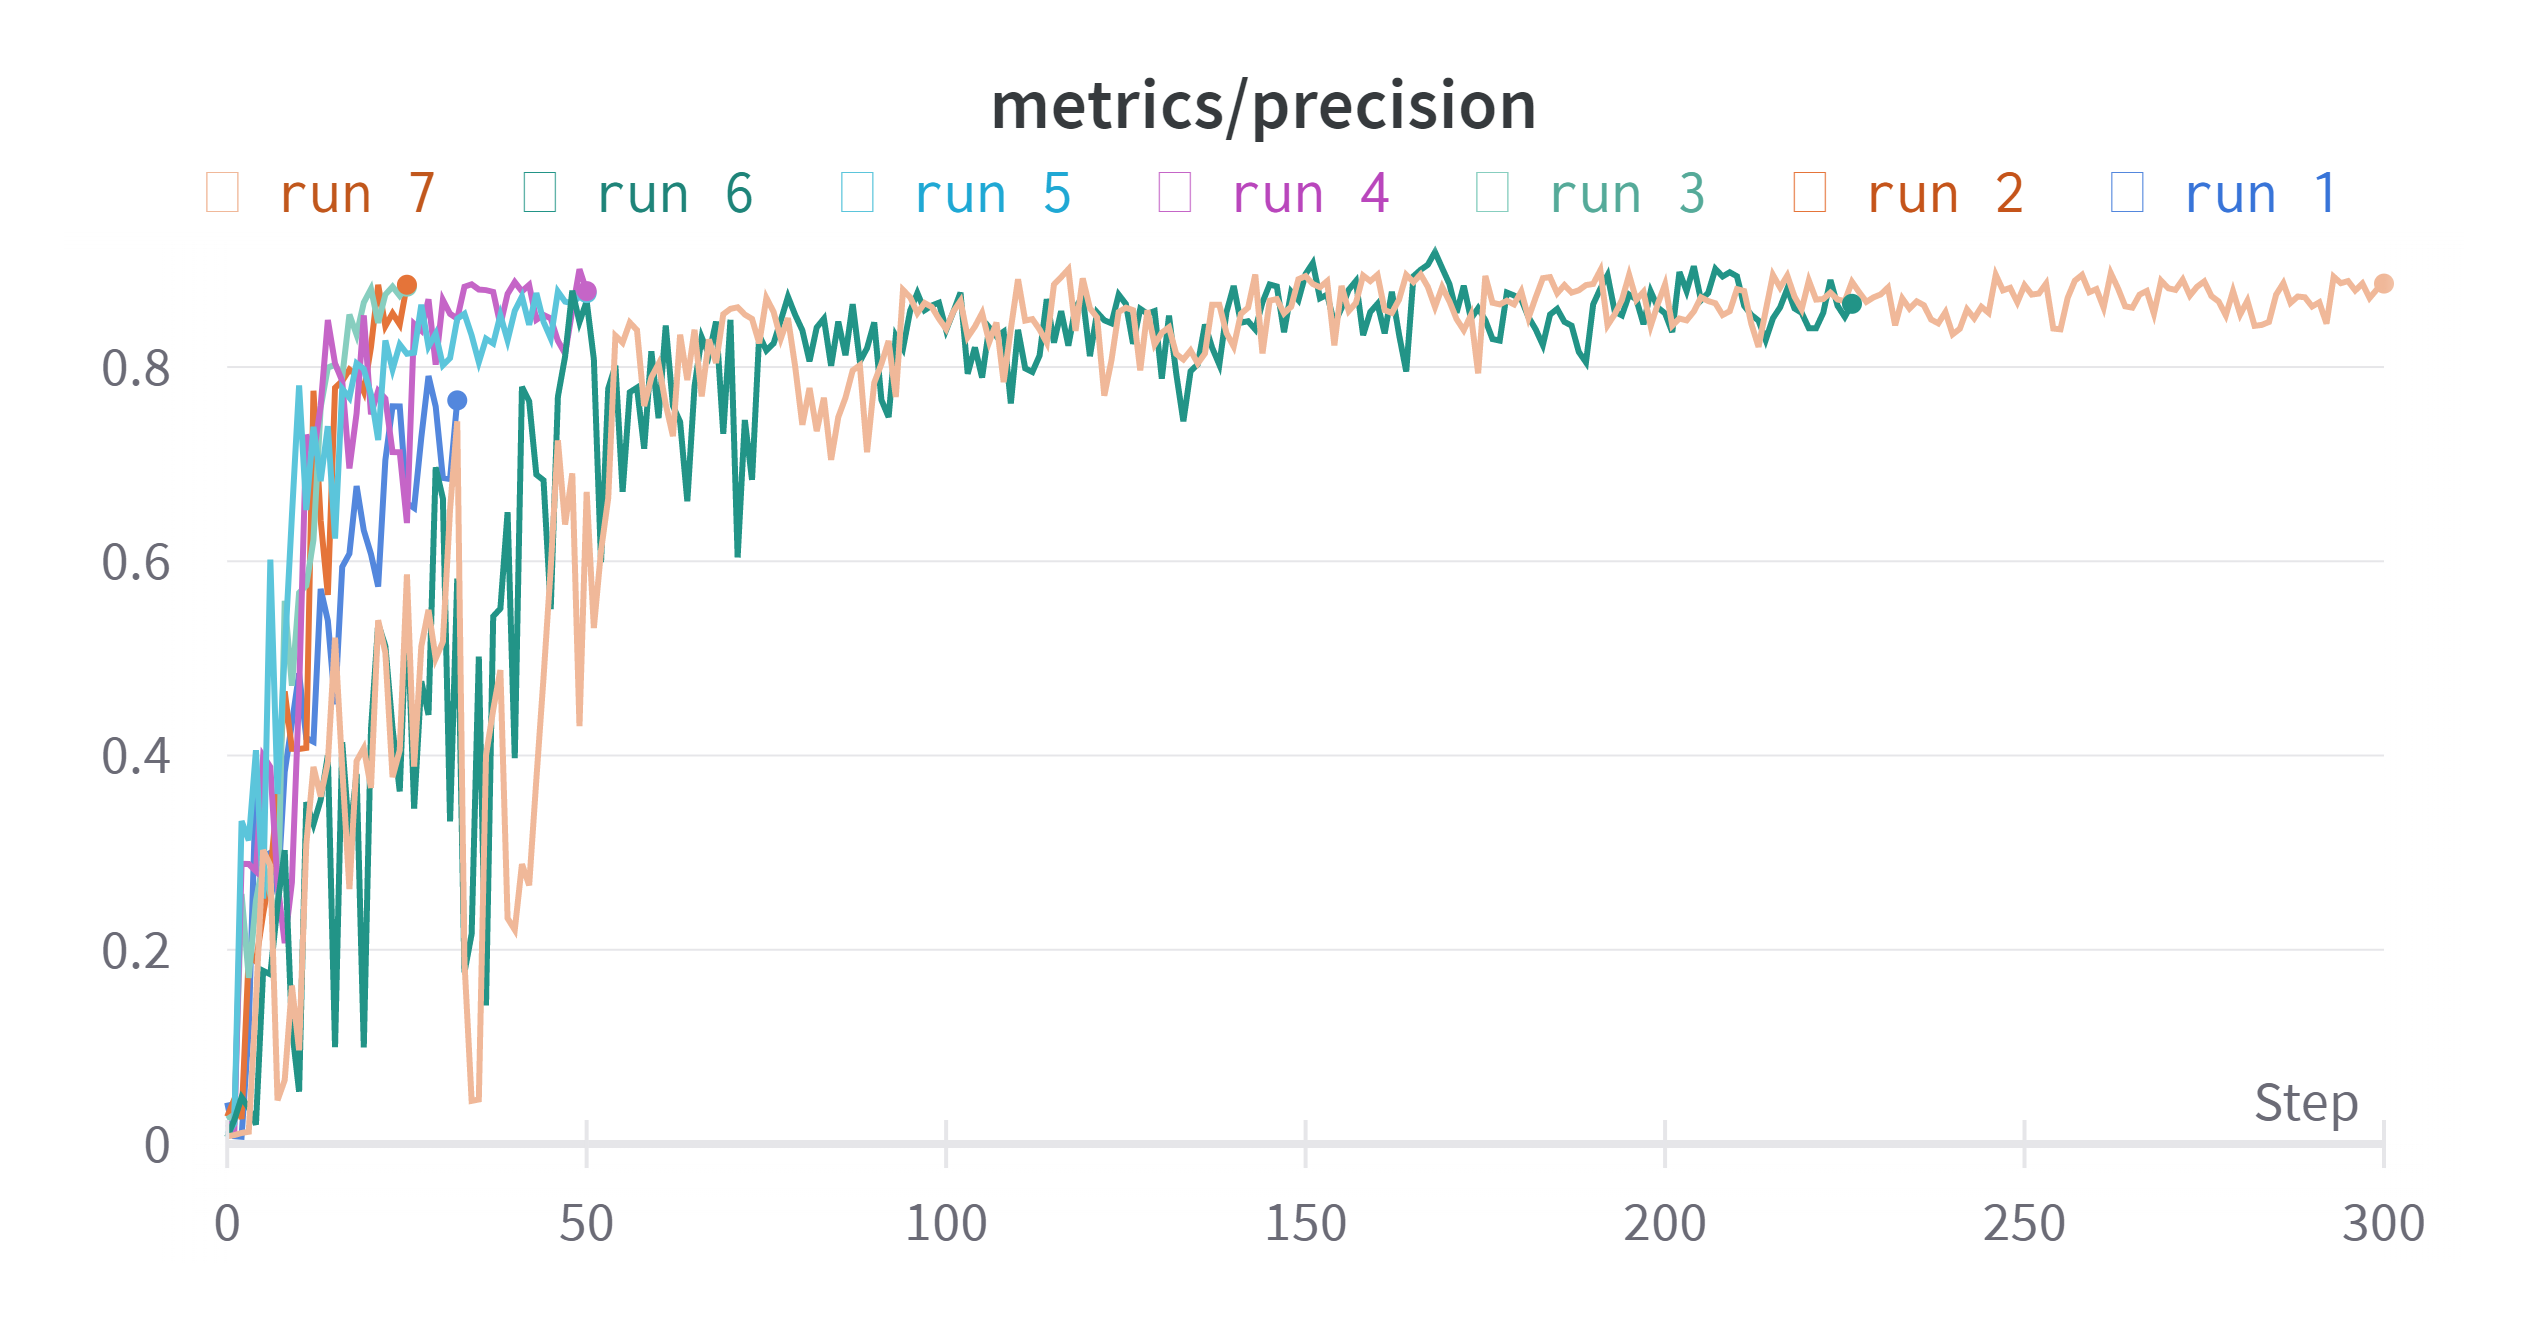
\includegraphics[width=0.8\textwidth]{images/05Testing/precision.png}
	\caption{precision}
	\label{precision}
\end{figure}

\begin{figure}[h!]
	\centering
	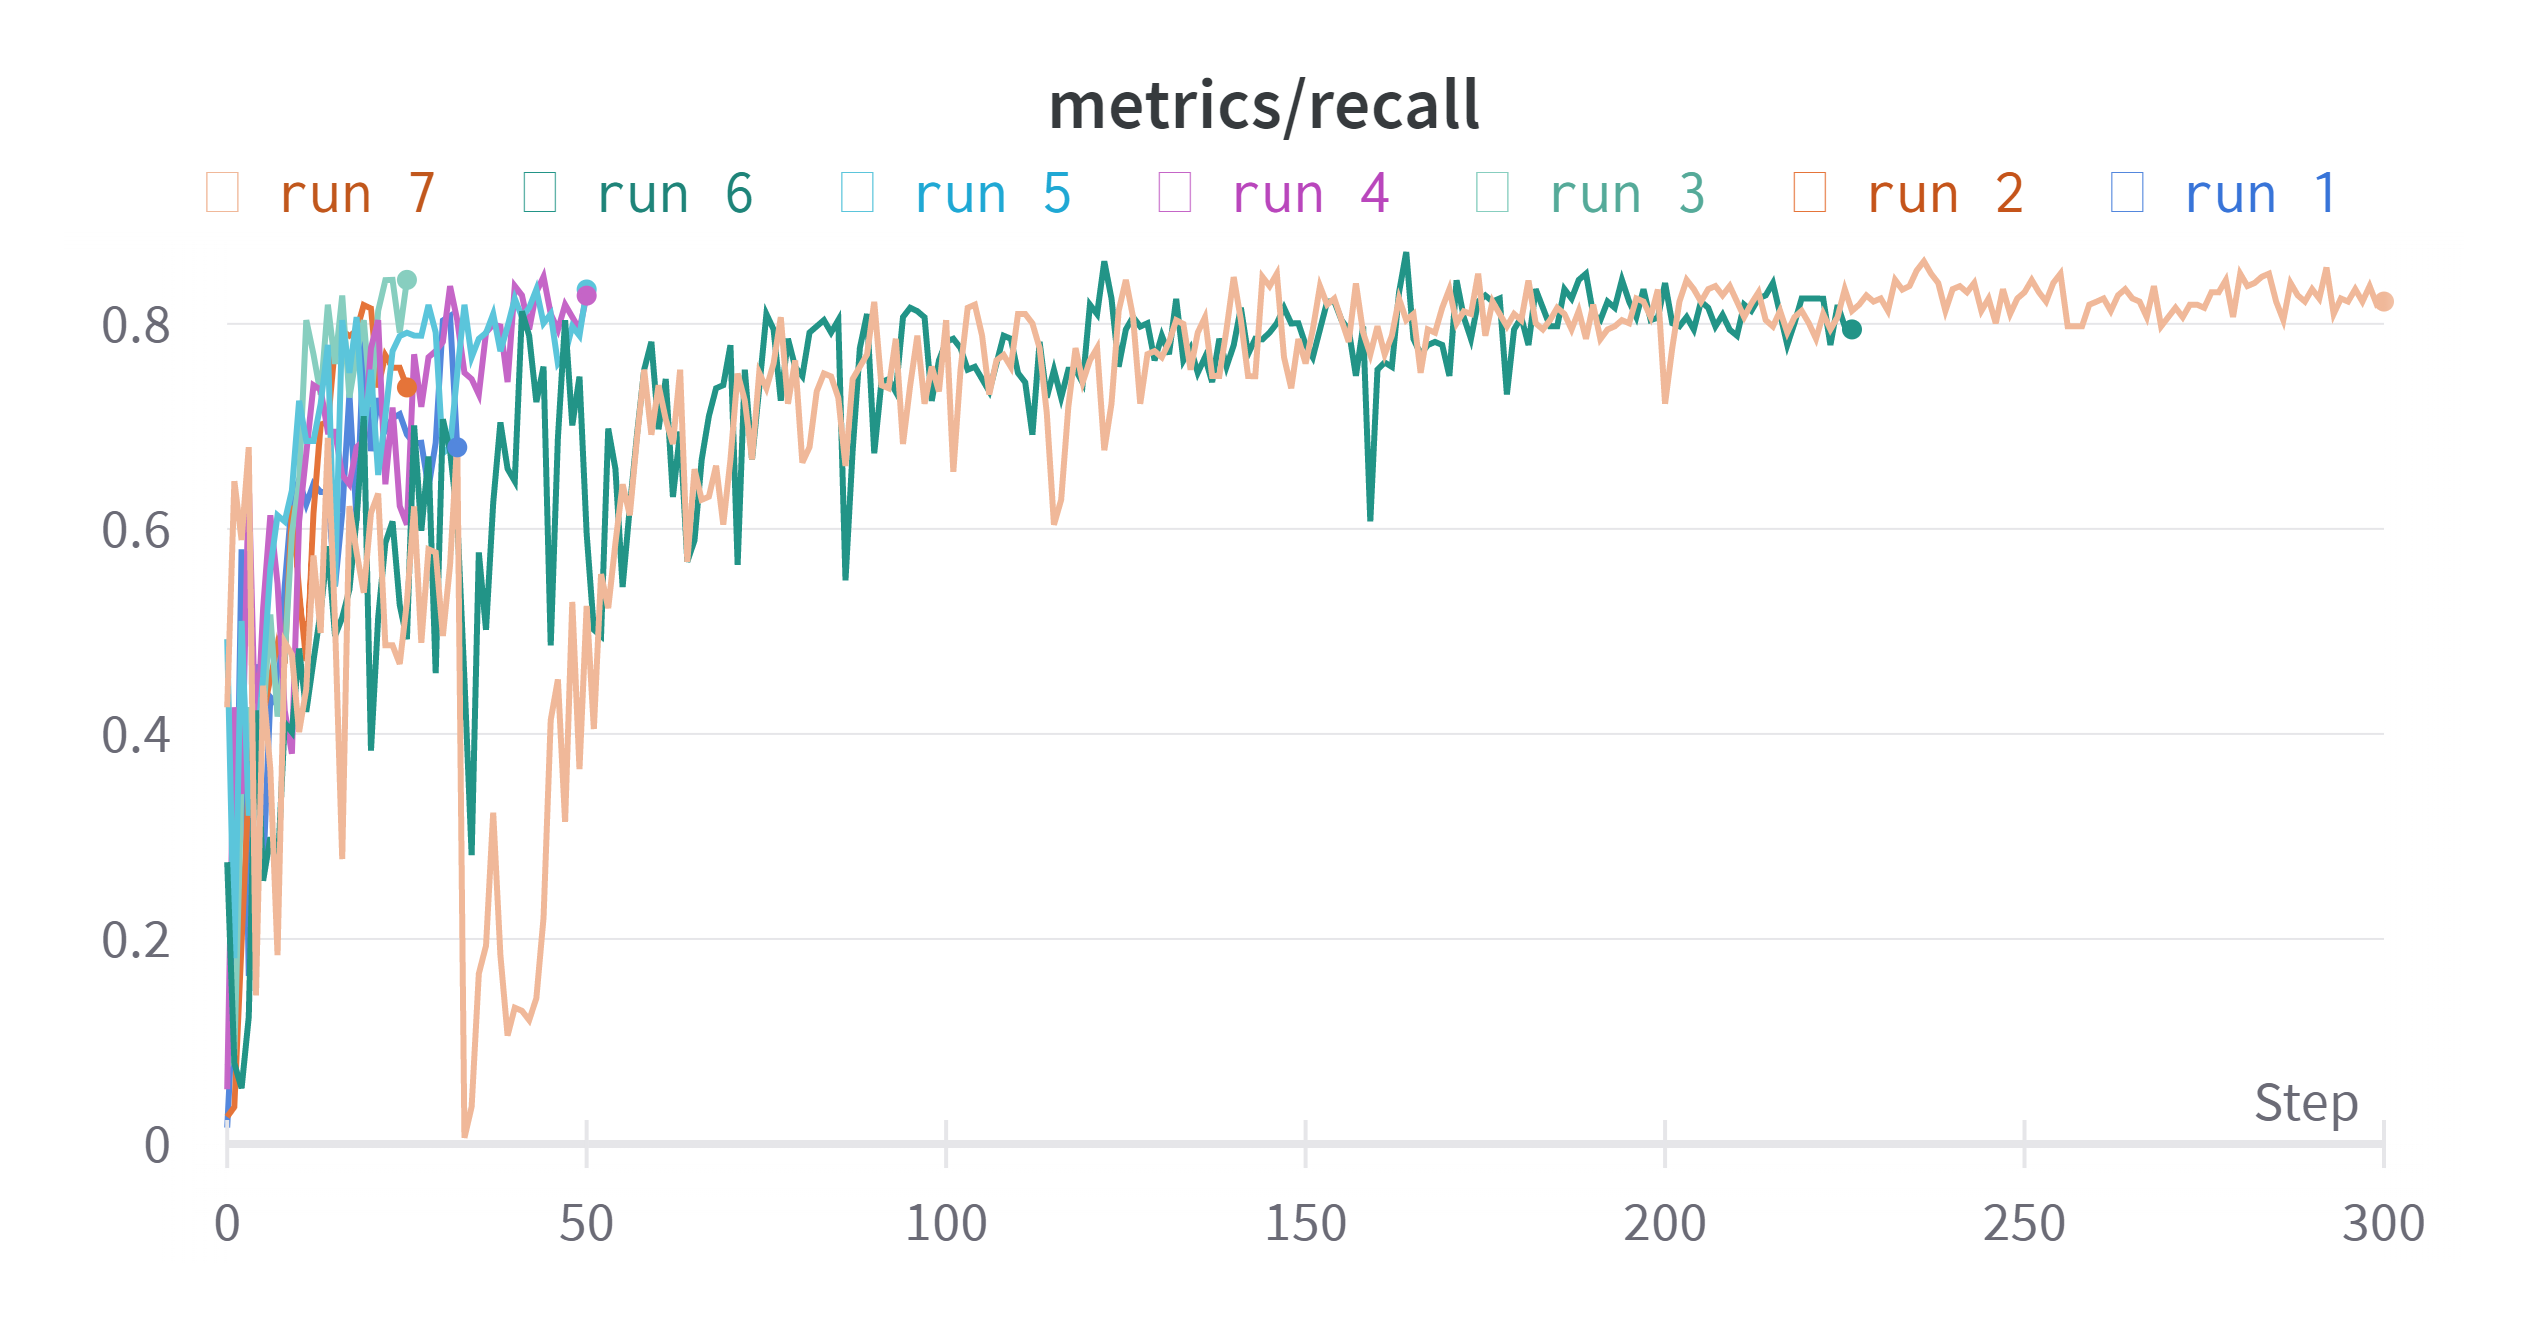
\includegraphics[width=0.8\textwidth]{images/05Testing/recall.png}
	\caption{recall}
	\label{recall}
\end{figure}

\section{Model 1}
Experiment 1 commenced testing with disappointing results. The model consistently undercounted, detecting very few cells and demonstrating a count error of nearly 100\% (see Figure \ref{count_error}). This can be attributed to the model's poor localisation capabilities as seen in Figure \ref{model1}: few cells are detected, and those which are are predicted with low confidence. This suggested that the configuration for Experiment 1 was flawed, and did not allow the model to learn enough about the target class to make accurate predictions.\\

\begin{figure}
\subfloat{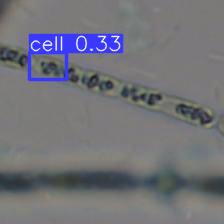
\includegraphics[width=3in]{images/05Testing/run01/easy}}
\subfloat{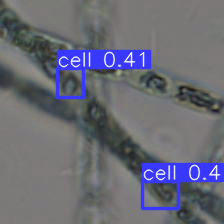
\includegraphics[width=3in]{images/05Testing/run01/hard}}
\caption{Predictions on 'easy' (left) and 'hard' (right) images from the test set by Model 1}
\label{model1}
\end{figure}

\section{Model 2}
The poor performance of Model 1 prompted a revision of the dataset annotations, which were revised from the sparse Version 1 to Version 2. Version 2 included far more cells, including those which were less clearly depicted. It was hypothesised that this change would provide the model with sufficient information to generalise across different levels of image clarity.\\

From Model 2 onwards, the undercounting problem was reversed: all models following Model 1 consistently \textit{over}counted, initially with errors of more than 100\%. This reversal cannot be attributed to one change alone between Experiments 1 and 2—both the batch size (16 to 32) and the number of epochs (32 to 25) were changed—but these changes were insignificant compared to the overhaul of the dataset annotations. It seemed that the resulting model was highly vulnerable to producing false positives and counting the same cells twice, and this was confirmed by qualitative evaluation of the model's predicted bounding boxes (see Figure \ref{model2}). This suggested that the revision of the dataset annotations was the most likely cause of the dramatic difference in count error between Models 1 and 2.\\

While the error for Model 2 was greater than that of Model 1, making Model 2 strictly the 'worse' model, it was also taken into account that the implications of deploying an undercounting model such as Model 1 would be more serious than one which overcounted, such as Model 2. While the revision of the dataset annotations was seen as the likely reason for Model 2's overcounting, it was decided to err on the side of more annotation, since overcounting is more desirable than undercounting.

\begin{figure}
\subfloat{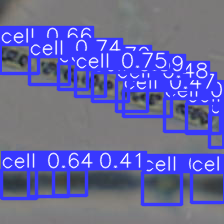
\includegraphics[width=3in]{images/05Testing/run02/easy}}
\subfloat{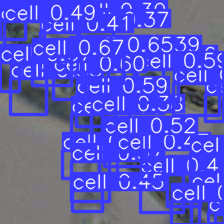
\includegraphics[width=3in]{images/05Testing/run02/hard}}
\caption{Predictions on 'easy' (left) and 'hard' (right) images from the test set by Model 2}
\label{model2}
\end{figure}

\section{Model 3}
For the third experiment, the proportion of the dataset used for training was increased by 20\% for a train/test/val split of 70/15/15. It was theorised that Model 2's overcounting problem might be ameliorated by providing the model with more data to learn from. In addition, the dataset annotations were revised to Version 3, which added cells which were both out-of-focus and not fully within the patch, and occluded cells.\\

This model showed marginal improvement in count error compared to Model 2. Since both of the changes to the configuration were made simultaneously, it is unclear whether either change, in isolation, might have yielded substantial improvement or deterioration. In particular, the significance of enlarging the training set could be investigated in isolation, since the previous revision to the dataset annotations yielded reduced accuracy. This might have counteracted any positive effect of the larger training set in this case.

\section{Model 4}
The only change made to the configuration for Experiment 4 was to increase the number of epochs (30 to 50). This resulted in a sharp reduction in count error, greater than that seen in Experiment 3. 

\begin{figure}
\subfloat{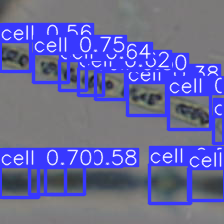
\includegraphics[width=3in]{images/05Testing/run04/easy}}
\subfloat{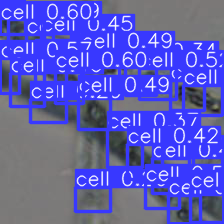
\includegraphics[width=3in]{images/05Testing/run04/hard}}
\caption{Predictions on 'easy' (left) and 'hard' (right) images from the test set by Model 4}
\label{model4}
\end{figure}

\section{Model 5}
Model 5 was fine-tuned on a significantly more complex base model than previous models (YOLOv5l). This change had a negligible benefit for numerical count error, and in fact increased count percentage count error.

\section{Model 6}
Experiment 6 dramatically increased the number of epochs (50 to 300) and batch size (32 to 128), after the success of Experiment 4 and on the recommendation of the YOLOv5 documentation\footnote{Tips for Best Training Results · ultralytics/yolov5 Wiki. (no date). Available at: https://github.com/ultralytics/yolov5/wiki/Tips-for-Best-Training-Results (Accessed: 05/05/2022).}. The base model was also changed back to YOLOv5s. These changes had the most dramatic effect on the model's count error of all those made during experimentation, resulting in substantial improvement.

\begin{figure}
\subfloat{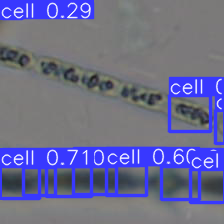
\includegraphics[width=3in]{images/05Testing/run06/easy}}
\subfloat{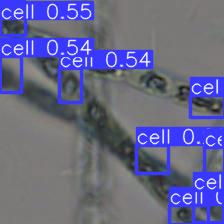
\includegraphics[width=3in]{images/05Testing/run06/hard}}
\caption{Predictions on 'easy' (left) and 'hard' (right) images from the test set by Model 6}
\label{model6}
\end{figure}

\section{Model 7}
Experiment 7 again changed the base model from YOLOv5s to YOLOv5l. Using this more complex model resulted in only marginally greater counting accuracy than the YOLOv5s-based Model 6.

\begin{figure}
\subfloat{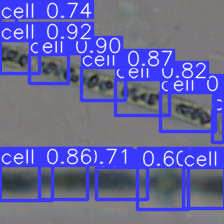
\includegraphics[width=3in]{images/05Testing/run07/easy}}
\subfloat{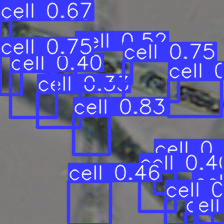
\includegraphics[width=3in]{images/05Testing/run07/hard}}
\caption{Predictions on 'easy' (left) and 'hard' (right) images from the test set by Model 7}
\label{model7}
\end{figure}